\bf{Пример 1}

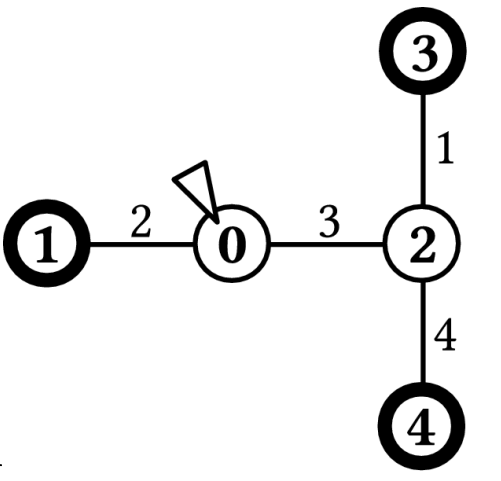
\includegraphics{crocodile1.png}

Комнаты показаны кружками, а коридоры, соединяющие их~--- отрезками. Комнаты с выходами обведены жирным контуром. Бенджама начинает движение в комнате с номером $0$ (она отмечена треугольником). Оптимальный план побега таков:

\begin{itemize}
\item Если ты когда-нибудь попадёшь в комнату с номером $0$, убегай по коридору, ведущему в комнату с номером $1$. Однако если этот коридор заблокирован, убегай по коридору, ведущему в комнату с номером $2$.
\item Если ты когда-нибудь попадёшь в комнату с номером $2$, убегай по коридору, ведущему в комнату с номером $3$. Однако если этот коридор заблокирован, убегай по коридору, ведущему в комнату с номером $4$.
\end{itemize}

В наихудшем случае Бенджама попадёт в комнату с выходом за $7$ единиц времени. Таким образом, процедура \t{travel\_plan} должна возвращать число $7$.

\bf{Пример 2}

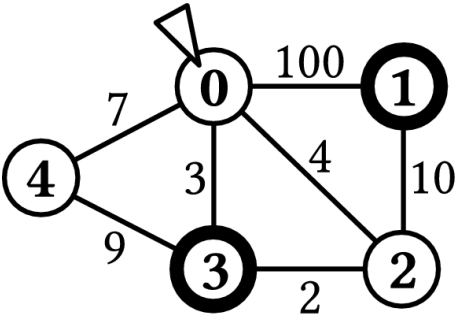
\includegraphics{crocodile2.png}

Оптимальный план побега описывается следующим образом:

\begin{itemize}
\item Если ты когда-нибудь попадёшь в комнату с номером $0$, убегай по коридору, ведущему в комнату с номером $3$. Однако если этот коридор заблокирован, убегай по коридору, ведущему в комнату с номером $2$.
\item Если ты когда-нибудь попадёшь в комнату с номером $2$, убегай по коридору, ведущему в комнату с номером $3$. Однако если этот коридор заблокирован, убегай по коридору, ведущему в комнату с номером $1$.
\item Не беспокойся насчёт комнаты с номером $4$~--- по плану ты никогда не попадёшь в неё.
\end{itemize}

Бенджама попадёт в какую-либо из комнат с выходом не позже, чем по прошествии $14$ единиц времени. Поэтому процедура \t{travel\_plan} должна возвращать значение $14$.
